\subsubsection{18.11.14}

\begin{enumerate}
	\item The time of beginning and ending of the meeting:
	16:00 - 1:00
	\item Purposes of the meeting:
	\begin{enumerate}
	  \item To train on the control of robot.
	  
    \end{enumerate}
    
	\item Work, that has been done:
	\begin{enumerate}
	  \item The first tests of the robot showed the failure of the idea installation inside the tube plastic bottle. It reduced internal diameter so the balls stuck in the pipe. It was decided to remove the bottle. It solved this problem but now the length of tube is too small for throwing of balls to baskets.
      
      \item It was turned out that MOB can't turn the bucket when it filled with balls. It was installed fishing cargo mass 100g on the top part of bucket. So this problem was solved.
      
      \begin{figure}[H]
      	\begin{minipage}[h]{0.2\linewidth}
      		\center   
      	\end{minipage}
      	\hfill
      	\begin{minipage}[h]{0.27\linewidth}
      		\center{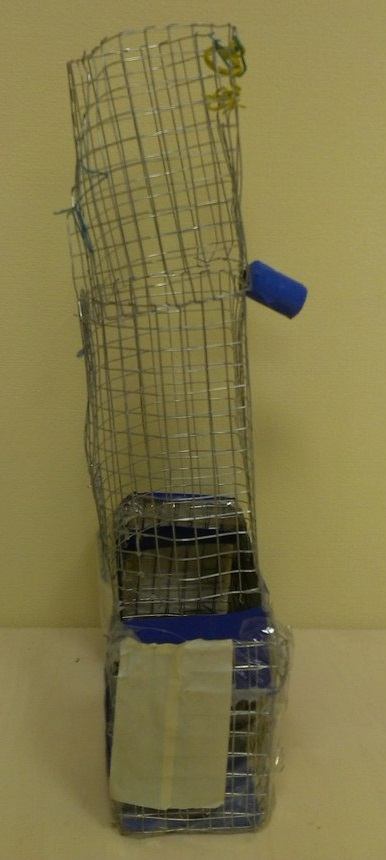
\includegraphics[scale=0.25]{days/18.11.14/images/01}}  
      	\end{minipage}
      	\hfill
      	\begin{minipage}[h]{0.27\linewidth}
      		\center{
\includegraphics[scale=0.22]{days/18.11.14/images/02}}
      	\end{minipage}
      	\hfill
      	\begin{minipage}[h]{0.2\linewidth}
      		\center  
      	\end{minipage}
      	\caption{Fishing cargo on bucket}
      \end{figure}
      
      \item Also it was turned out that two motors can't extract the lift. Fuses are heated and unlock the chain so the operator loses the control of lift. It was decided install transmission with the gear ratio 1:2 for reducing of load to motors .
      
     % \begin{figure}[H]
     % 	\begin{minipage}[h]{0.2\linewidth}
     % 		\center  
     % 	\end{minipage}
     % 	\begin{minipage}[h]{0.6\linewidth}
     % 		\center{
\includegraphics[scale=0.3]{days/18.11.14/images/03}}
     % 		\caption{Механизм лебедки с передаточным отношением 1:2}
     % 	\end{minipage}
     % \end{figure}
      
      \item Motors copes with extracting the lift after installation of transmission but sometimes the lift was jammed. It happens due to the clamping of the belt between top crossbar of the bottom slat and bottom crossbar of the second slat. It was decided to install limiters that will not allow to bottom crossbar of the second slat raise too highly.
          
    \end{enumerate}
    
	\item Results:
	\begin{enumerate}
	  \item Plastic bottles were removed from the bucket. 
	  
      \item It was installed transmission with the ratio 1:2 on the motors which extracts the lift .
      
      \item It was installed the cargo for normaly working of MOB.
    \end{enumerate}
    
	\item Tasks for the next meetings:
	\begin{enumerate}
	  \item To install the limiters of moving of crossbar at the lift.
	  
	  \item To extend the tube of bucket for throwing of balls to baskets.
	  
	  \item To train on the control of robot.

    \end{enumerate}     
\end{enumerate}
\fillpage